\documentclass[12pt,a4paper]{article}
\usepackage{mainsty}
\begin{document}

\begin{center}
  \large\textsc{\imp{Induction \& Recursion}}
\end{center}
\begin{enumerate}
  \item \topic{Sequences} is a special type of function in which the domain is a set of consecutive integers.
  A geometric sequence is a sequence of real numbers where each term after the initial term is found by taking the previous term and multiplying by a fixed number called the common ratio. A geometric sequence can be finite or infinite.
  \begin{itemize}
    \item Increasing and non-decreasing
    \item[] 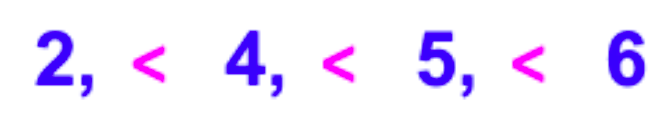
\includegraphics[scale=0.5]{seq1}
    \item Non-decreasing but non increasing
    \item[] 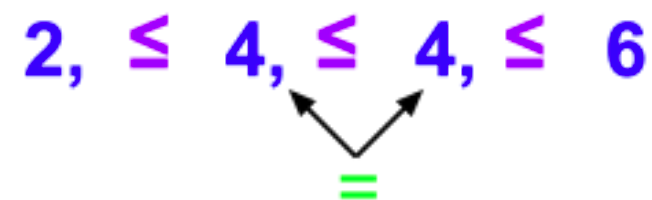
\includegraphics[scale=0.5]{seq2}
  \end{itemize}
  \item \topic{Recurrence relations} Some sequences are most naturally defined by specifying one or more initial terms and then giving a rule for determining subsequent terms from earlier terms in the sequence. A rule that defines a term an as a function of previous terms in the sequence is called a recurrence relation.
  \begin{itemize}
    \item Given the definition of a sequence \(f_{n}\) whose domain is the set of all non-negative integers:\\
    \(f_{0} = 2\) \\
    \(f_{1} = 3\) \\
    \(f_{n} = f_{n-2} \cdot f_{n-1}\), for \(n \geq 2\) \\
    \(f_{2} = f_{0} \cdot f_{1} = 6\) \\
    \(f_{3} = f_{1} \cdot f_{2} = 18\) \\ 
    \(f_{4} = f_{2} \cdot f_{3} = 108\) \\
    \(f_{5} = f_{3} \cdot f_{4} = 1944\)
  \end{itemize}
  \item \topic{Summations}
  \begin{itemize}
    \item[] \(\displaystyle\sum_{i = 1}^{10} (i + 5) \) = \(\displaystyle\sum_{i = 1}^{?} (i + 5) + (?) \)
    \item[] \(\displaystyle\sum_{i = 1}^{10} (i + 5) \) = (1 + 5) + (2 + 5) + \(\ldots \) + (10 + 5)
    \item[] \(\displaystyle\sum_{i = 1}^{10} (i + 5) \) = [(1 + 5) + (2 + 5) + \(\ldots \)] + (10 + 5)
    \item[] \(\displaystyle\sum_{i = 1}^{10} (i + 5) \) =  \(\displaystyle\sum_{i = 1}^{9} (i + 5) \) + (15)
    \item Enter the result of the sum of the first 6 terms in the geometric sequence with initial term a = 10, and common ratio r = 4.
    \item[] \(\displaystyle\sum_{j=0}^{5} (10 \cdot 4^{j}) = ? \)
    \item[] \(\displaystyle\sum_{j=0}^{n-1} (a \cdot r^j) = \frac{a(r^n-1)}{r-1} \)
    \item[] \(\displaystyle\sum_{j=0}^{5} (10 \cdot 4^j) = \frac{10(4^6-1)}{4-1} = \frac{40950}{3} = 13650 \)
    \item Enter the result of the sum of the first 25 terms in the arithmetic sequence with initial term a = 1, and common difference d = 5.
    \item[] \(\displaystyle\sum_{j=0}^{24} (1 + 5j) = ? \) 
    \item[] \(\displaystyle\sum_{j=0}^{n-1} (a + jd) = an + \frac{d(n-1)n}{2} \) 
    \item[] \(\displaystyle\sum_{j=0}^{24} (1 + 5j) = 1\cdot 25 + \frac{5 \cdot (24)  \cdot 25}{2} = 25 + \frac{3000}{2} = 25 + 1500 = 1525\) 
  \end{itemize}
  \item \topic{Mathematical induction} 
  \begin{itemize}
    \item Theorem: For every positive integer n, \(\displaystyle\sum_{j=1}^{n} j = \frac{n(n+1)}{2} \)
    \item Proof. By induction on n.
    \item Base Case: n = 1
    \item[] When n = 1, the left side of the equation is \(\displaystyle\sum_{j=1}^{1} j = 1\) 
    \item[] When n = 1, the right side of the equation is \(\frac{1(1+1)}{2} = 1\)
    \item[] Therefore, \(\displaystyle\sum_{j=1}^{1} j = \frac{1(1+1)}{2}\)
    \item Inductive step: Suppose that for positive integer k, \(\displaystyle\sum_{j=1}^{k} j = \frac{k(k+1)}{2}\), then we show that \(\displaystyle\sum_{j=1}^{k+1} j = \frac{k(k+1)(k+2)}{2}\)
    \item Starting with the left side of the equation to be proven:
    \item[] \(\displaystyle\sum_{j=1}^{k+1} j = \displaystyle\sum_{j=1}^{k} j + (k + 1)\), by separating out the last term
    \item[] \(\displaystyle\sum_{j=1}^{k+1} j = \frac{k(k+1)}{2} + (k + 1) \), by the inductive hypothesis
    \item[] \(\displaystyle\sum_{j=1}^{k+1} j = \frac{k(k+1) + 2(k+1)}{2} \)
    \item[] \(\displaystyle\sum_{j=1}^{k+1} j = \frac{(k + 2)(k + 1)}{2} \), by algebra
    \item Therefore, \(\displaystyle\sum_{j=1}^{k+1} j = \frac{(k+1)(k+2)}{2} \) 
  \end{itemize}
  \item \topic{Strong induction and well-ordering}
  \begin{itemize}
    \item[] 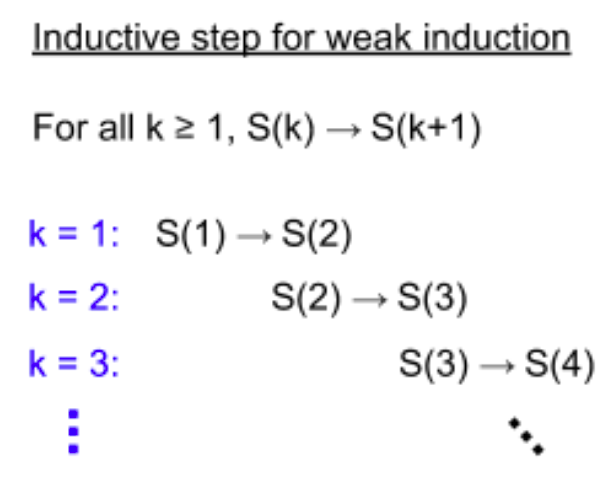
\includegraphics[scale=0.5]{weak}
    \item[] 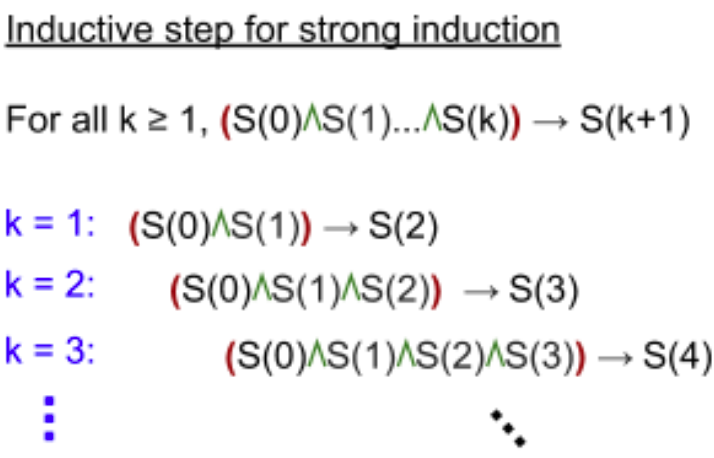
\includegraphics[scale=0.5]{strong}
  \end{itemize}
  \item \topic{Loop invariants} 
  \begin{itemize}
    \item The field of \textbf{program verification} is concerned with formally proving that programs perform correctly. 
    \item A program's correct behavior is defined by stating that if a \textbf{pre-condition} is true before the program starts, then the program will end after a finite number of steps and a \textbf{post-condition} is true after the program ends.
  \end{itemize}
  \item \topic{Recursive definitions} 
  \begin{itemize}
    \item In a \textbf{recursive definition} of a function, the value of the function is defined in terms of the output value of the function on smaller input values.
    \item A \textbf{basis} explicitly states that one or more specific elements are in the set.
    \item A \textbf{recursive rule} shows how to construct larger elements in the set from elements already known to be in the set. (There is often more than one recursive rule).
    \item An \textbf{exclusion statement} states that an element is in the set only if it is given in the basis or can be constructed by applying the recursive rules repeatedly to elements given in the basis.
    \item \textbf{Basis}: A single vertex with no edges is a perfect binary tree. The root is the only vertex in the tree.
    \item[] 
\includegraphics[scale=0.5]{recursive}
    \item \textbf{Recursive rule}: If T is a perfect binary tree, then a new perfect binary tree T' can be constructed by taking two copies of T, adding a new vertex v and adding edges between v and the roots of each copy of T. The new vertex v is the root of T'.
    \item[] 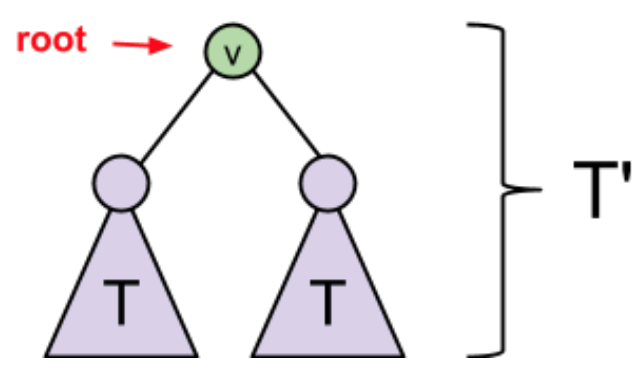
\includegraphics[scale=0.5]{recursive1}
  \end{itemize}
  \item \topic{Structural induction}
  \begin{itemize}
    \item \textbf{Structural induction} is a type of induction used to prove theorems about recursively defined sets that follows the structure of the recursive definition.
  \end{itemize}
  \item \topic{Recursive algorithms}
  \begin{itemize}
    \item A \textbf{recursive algorithm} is an algorithm that calls itself. Like recursively defined sequences and structures, a recursively defined algorithm has a base case in which the output is computed directly on an input of small size or value. On a larger input, the algorithm calls itself on an input of smaller size and uses the result to construct a solution to the larger input. An algorithm's calls to itself are known as \textbf{recursive calls}.
    \item Recursive algorithm to compute the factorial function.
    \item[] 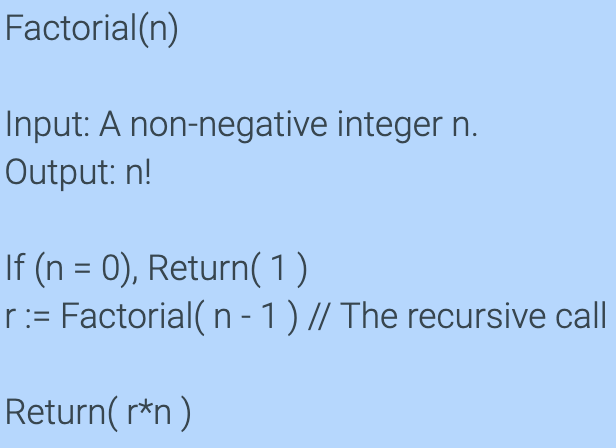
\includegraphics[scale=0.5]{fac} 
    \item Recursive algorithm to compute the power set of a set.
    \item[] 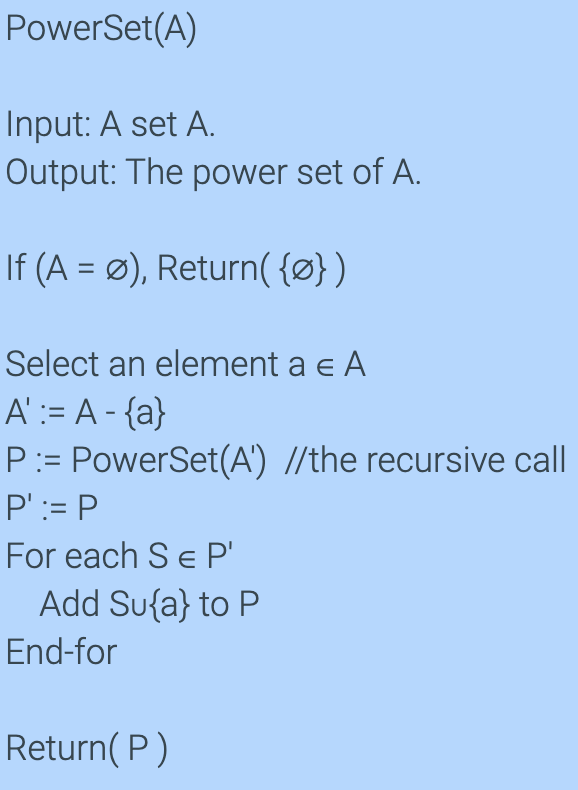
\includegraphics[scale=0.5]{set} 
    \item Recursive algorithm to compute Fibonacci numbers.
    \item[] 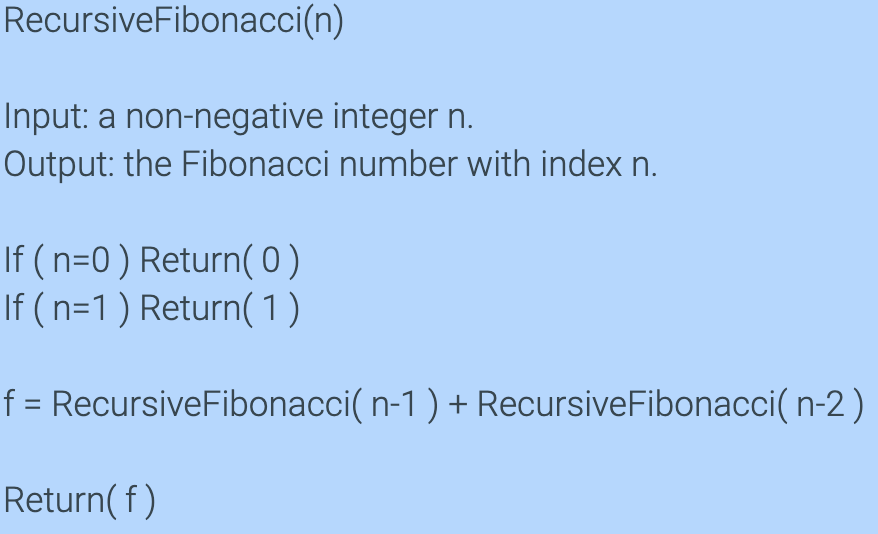
\includegraphics[scale=0.5]{fib} 
  \end{itemize}
  \item \topic{Analyzing the time complexity of recursive algorithms}
  \begin{itemize}
    \item The \textbf{time complexity} of an algorithm is a function \(T(n)\) indicating the number of atomic operations performed by the algorithm on an input of size n.
    \item \(Factorial(n)\): for \(n \geq 1\), \(T(n) = T(n-1) + \theta (1)\) 
  \end{itemize}
  \clearpage
  \item \topic{Divide-and-conquer algorithms: Introduction and mergesort}
  \begin{itemize}
    \item[] 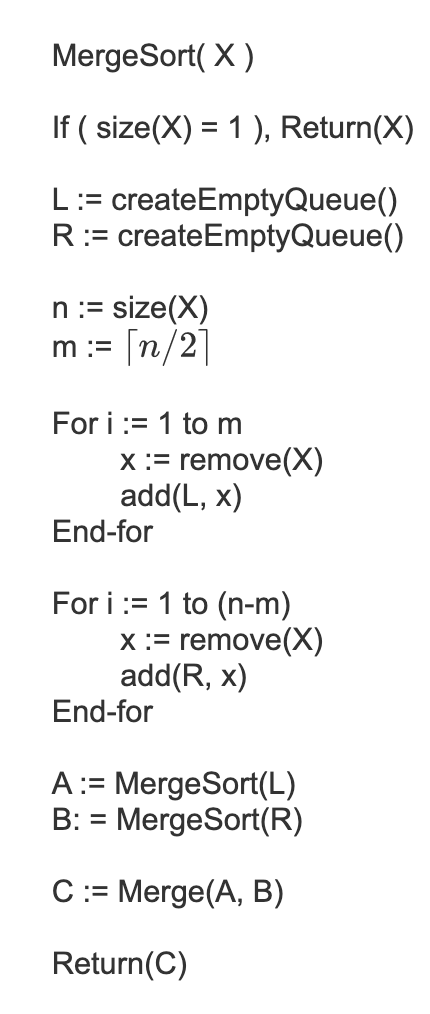
\includegraphics[scale=0.5]{merge}
    \item[] 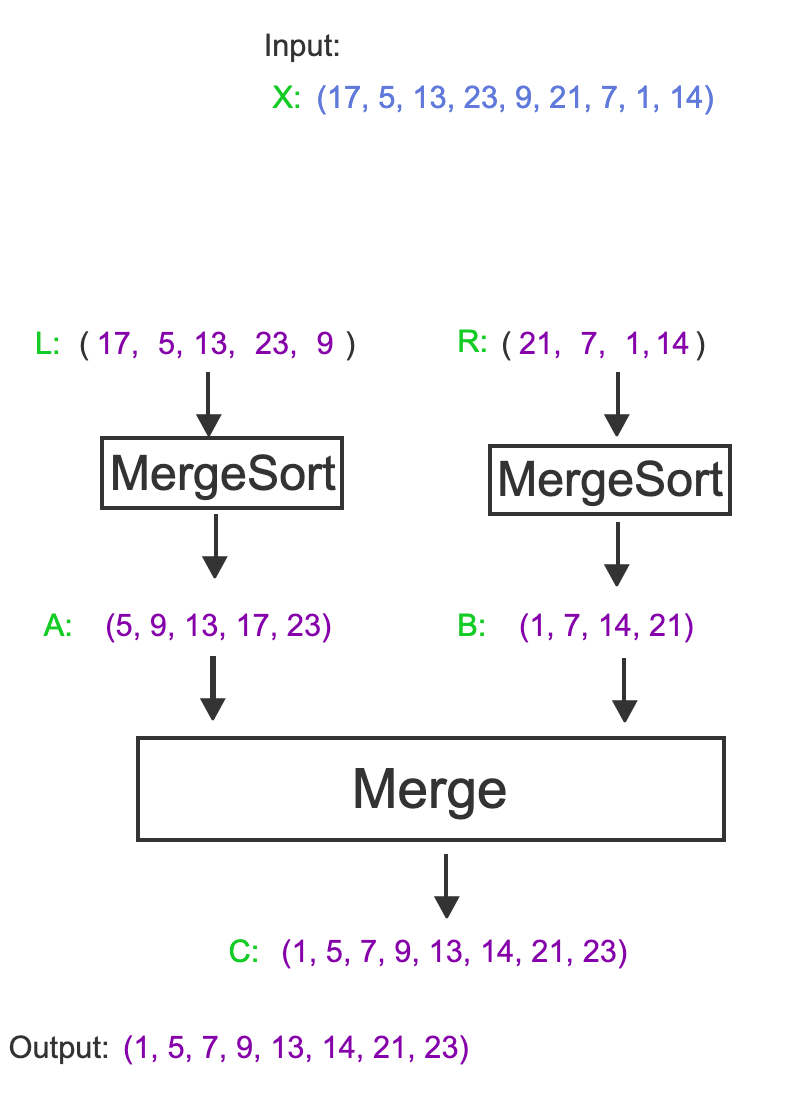
\includegraphics[scale=0.5]{merge1}  
  \end{itemize}
  \clearpage
  \item \topic{Divide-and-conquer algorithms: Binary search}
  \begin{itemize}
    \item[] 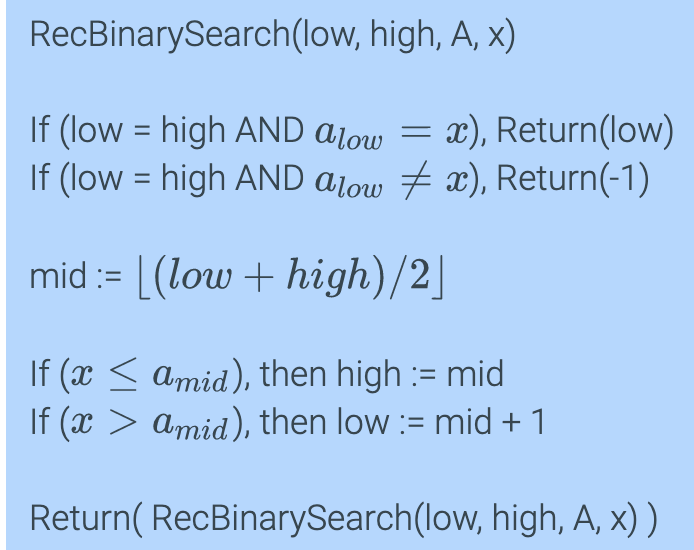
\includegraphics[scale=0.5]{binary} 
  \end{itemize}
  \item \topic{Solving linear homogeneous recurrence relations}
  \begin{itemize}
    \item A linear homogeneous recurrence relation of degree k has the following form:
    \item[] \(f_n = c_1 f_{n-1} + c_2 f_{n-2} + \cdots + c_k f_{n-k} \), 
    \item[] where the \(c_j\)'s are constants that do not depend on n, and \(c_k \neq 0\). 
    \item[] 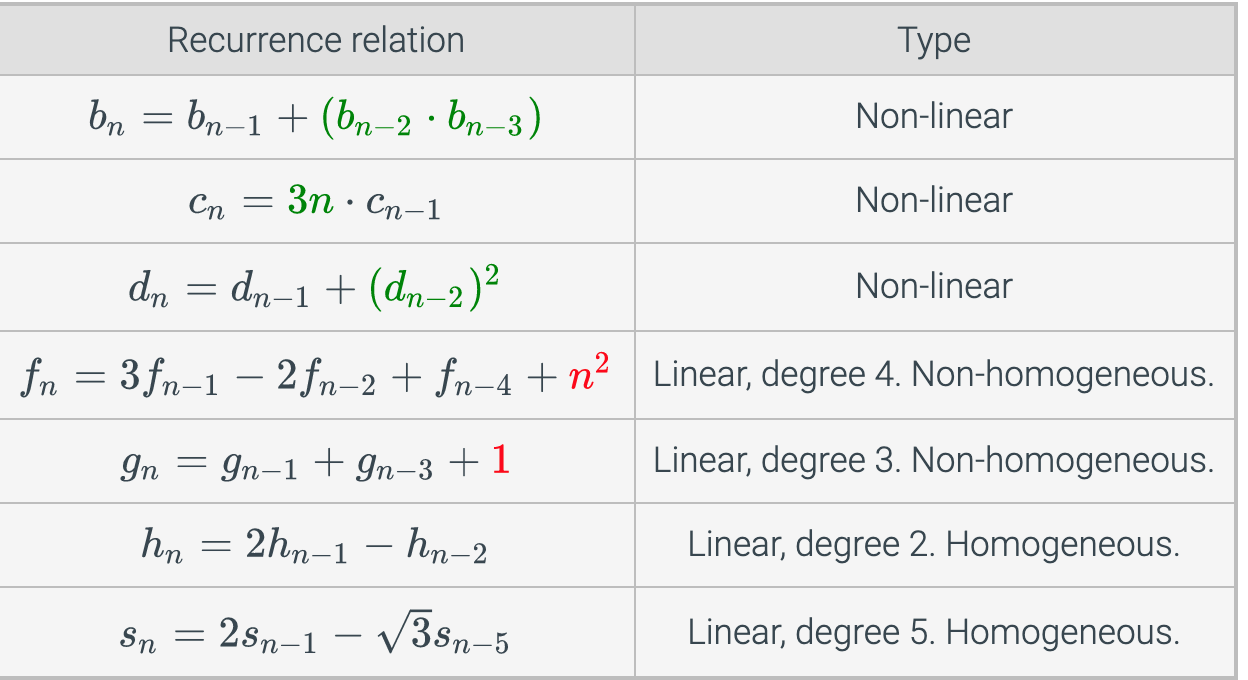
\includegraphics[scale=0.5]{chart} 
    \item[] 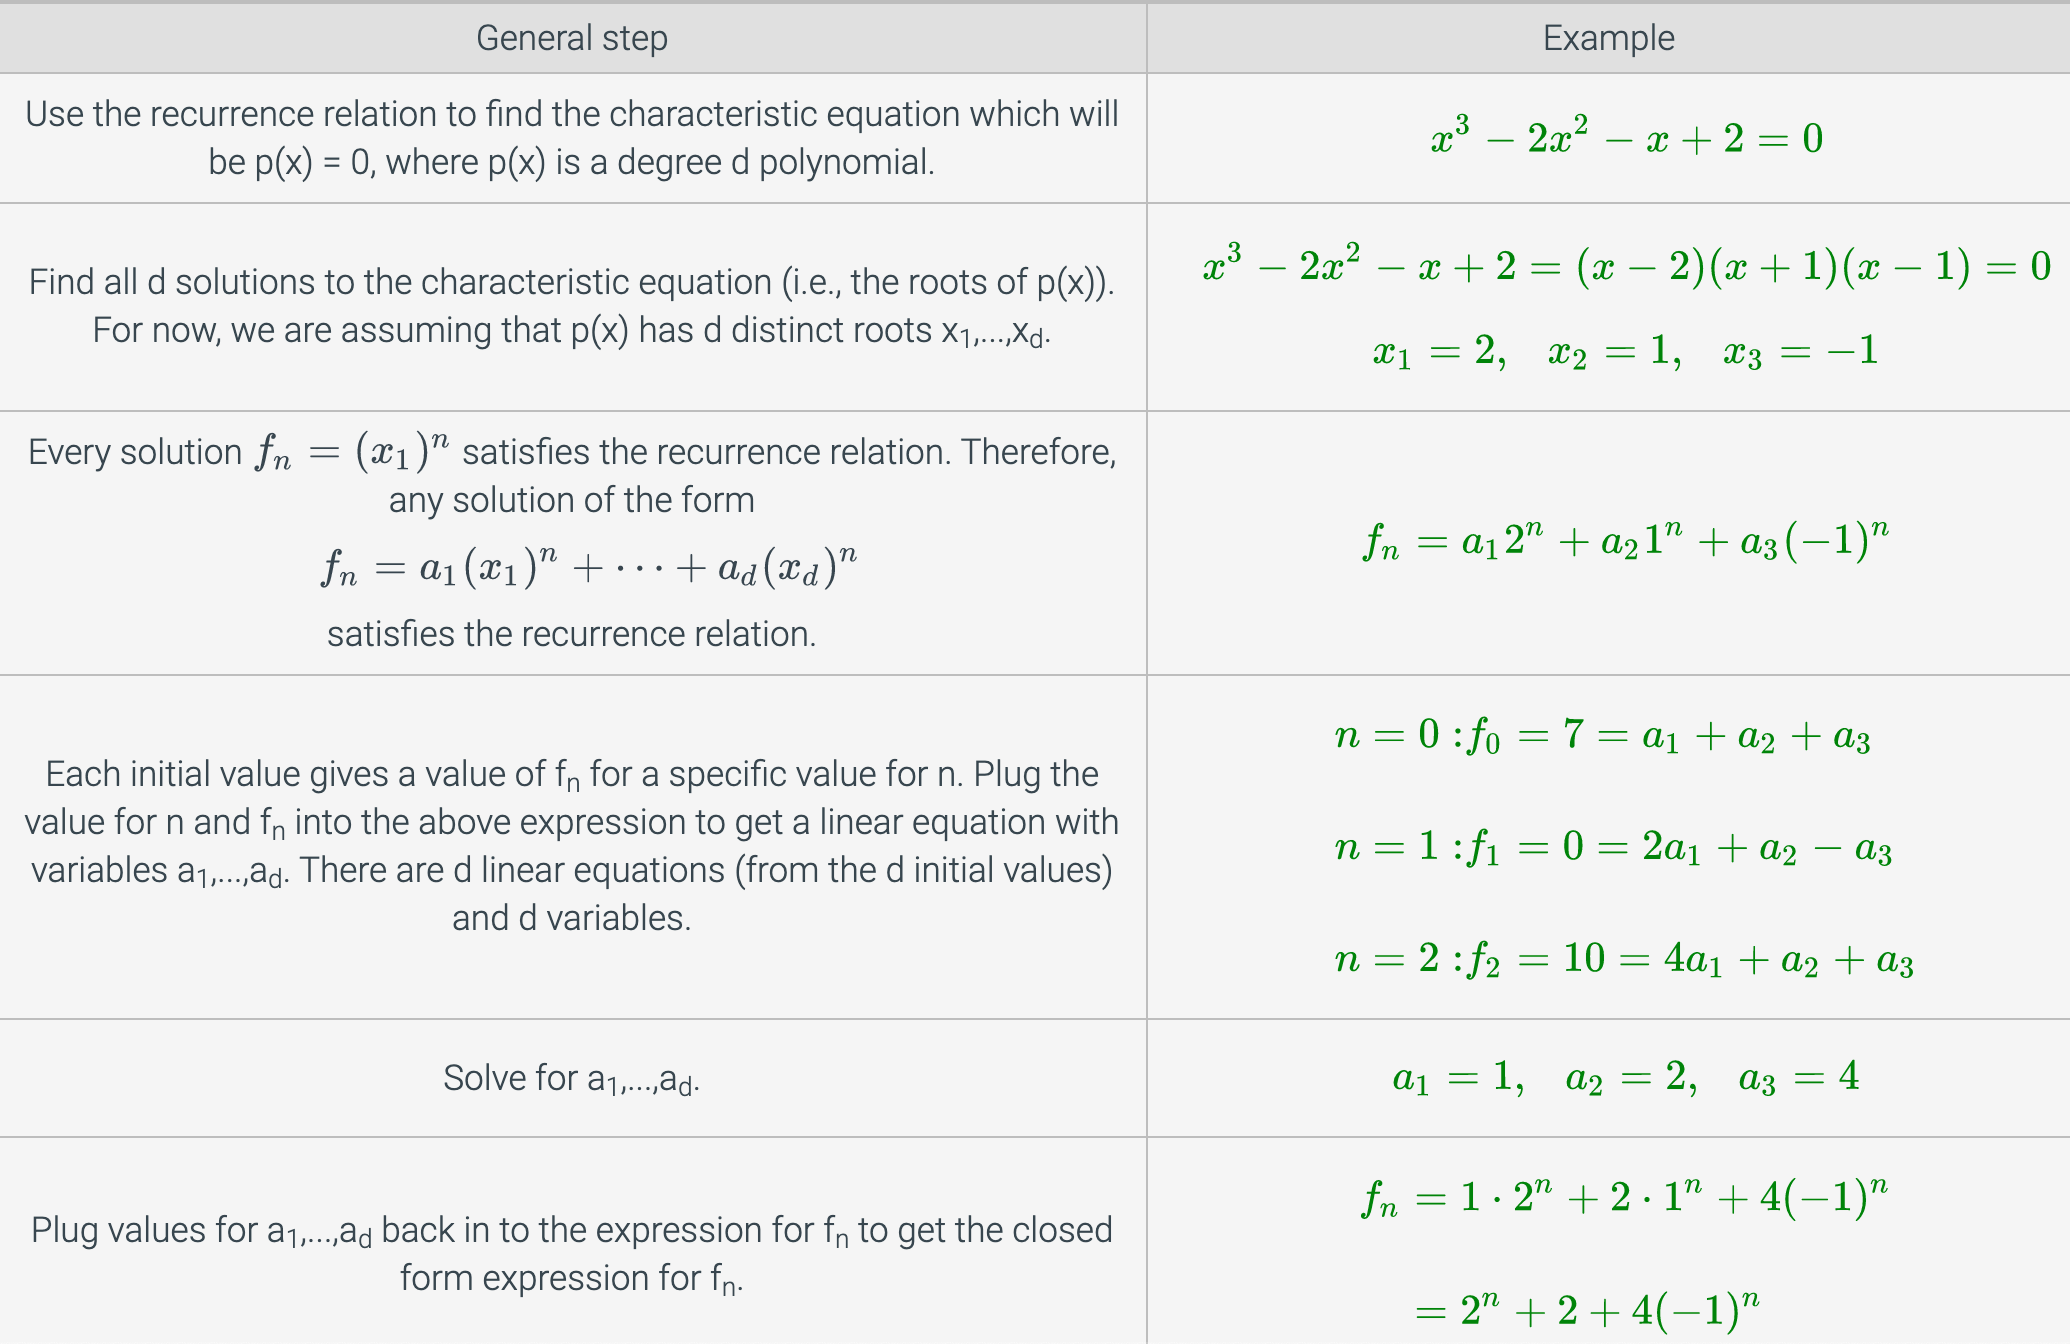
\includegraphics[scale=0.35]{chart1} 
  \end{itemize}
  \clearpage
  \item \topic{Solving linear non-homogeneous recurrence relations}
  \begin{itemize}
    \item A \textbf{non-homogeneous} linear recurrence relation is a linear recurrence relation with additional terms that are either a constant or a function of n. 
    \item[] 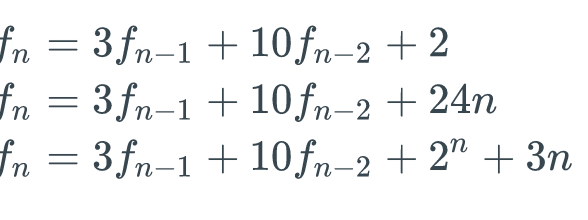
\includegraphics{non-home} 
    \item[] 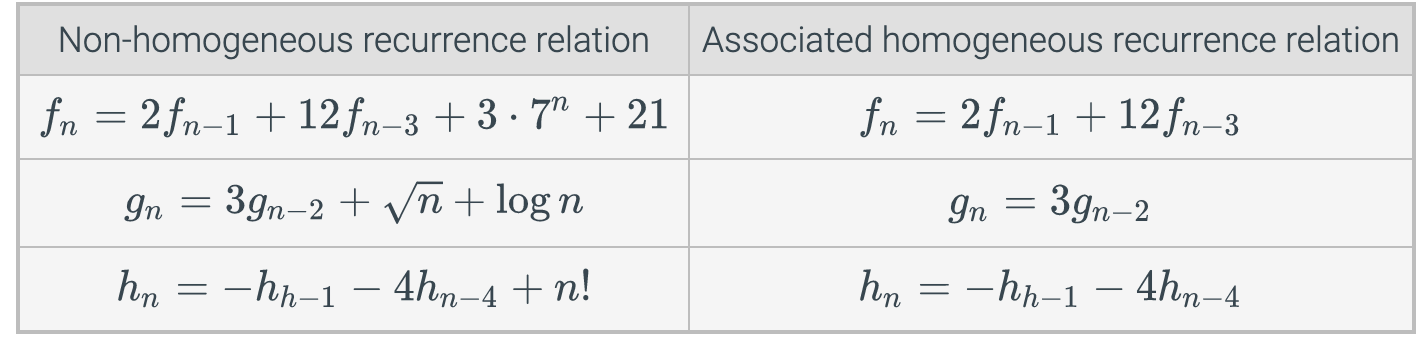
\includegraphics[scale=0.5]{non-homo} 
  \end{itemize}
  \item \topic{Divide-and-conquer recurrence relations}
  \begin{itemize}
    \item \(T(n) = aT(\frac{n}{b}) + \theta (n^d)\)
    \item[] 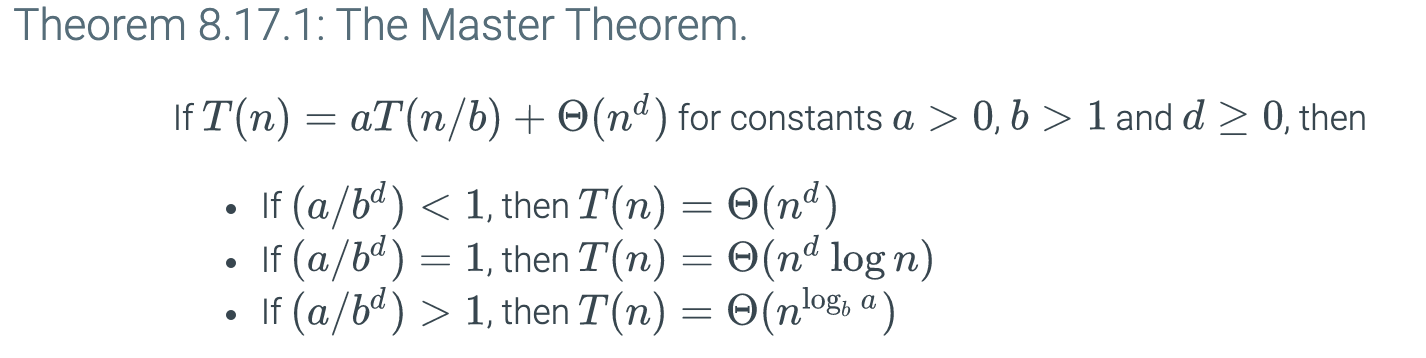
\includegraphics[scale=0.5]{master}
  \end{itemize}
\end{enumerate}


\clearpage
\begin{center}
  \large\textsc{\imp{Integer Properties}}
\end{center}
\begin{enumerate}
  \item \topic{The Division Algorithm}
  \begin{itemize}
    \item[] Compute the value of 24 div 5 = \boxed{4}
    \item[] Compute the value of -86 div 8 = \boxed{-11} \(\cdot \) 8 + 2 
    \item[]  Compute the value of 21 mod 4 = 5 \(\cdot \) 4 + \boxed{1}
    \item[]  Compute the value of -96 mod 9 = -11 \(\cdot \) 9 + \boxed{3} 
  \end{itemize}
  \item \topic{Modular arithmetic} 
  \begin{itemize}
    \item Compute the value of [(35 mod 8) + (38 mod 8)] mod 8
    \item[] [(3) + (6)] mod 8 = [1] mod 8 = \boxed{1}
    \item Compute the value of [67 \(\cdot \) 27] mod 5
    \item[] [(67 mod 5) (27 mod 5)] mod 5 = [(2) (2)] mod 5 = [4] mod 5 = \boxed{4}
    \item Compute the value of [67 \(\cdot \) 16 \(\cdot \) 73] mod 9
    \item[] [(67 mod 9) (16 mod 9) (73 mod 9)] mod 9 
    \item[] = [(4) (7) (1)] mod 9 
    \item[] = [(28) (1)] mod 9
    \item[] = [(28 mod 9) (1)] mod 9
    \item[] = [(1) (1)] mod 9 
    \item[] = [1] mod 9
    \item[] = \boxed{1}
    \item Compute the value of [71\(^{44}\) \(\cdot \) 14] mod 10
    \item[] [(71 mod 10)\(^{44}\) + 14] mod 10
    \item[] = [(1)\(^{44}\) + 14] mod 10 
    \item[] = [1 + 14] mod 10 
    \item[] = [15] mod 10
    \item[] = \boxed{5} 
  \end{itemize}
  \item \topic{Prime factorizations}
  \begin{itemize}
    \item A number p is \textbf{prime} if it is an integer greater than 1 and its only factors are 1 and p.
    \item A positive integer is \textbf{composite} if it has a factor other than 1 or itself.
    \item Every positive integer greater than one can be expressed as a product of primes called its \textbf{prime factorization}.
    \item A \textbf{non-decreasing} sequence is a sequence in which each number is equal to or greater than the one that came before.
    \item The \textbf{multiplicity} of a prime factor p in a prime factorization is the number of times p appears in the product of primes.
    \item The \textbf{greatest common divisor (gcd)} of non-zero integers x and y is the largest positive integer that is a factor of both x and y.
    \item The \textbf{least common multiple (lcm)} of non-zero integers x and y is the smallest positive integer that is an integer multiple of both x and y.
    \item Compute the prime factorization of: gcd\((12, 60)\)
    \item[] 12	=	\(2^2 \cdot 3^1 \cdot 5^0\), 60 = \(2^2 \cdot 3^1 \cdot 5^1\)
    \item[] gcd\((12,60)\) = \(2^2 \cdot 3^1 \cdot 5^0 = \boxed{2^2 \cdot 3}\) 
    \item Compute the prime factorization of: lcm\((18, 150)\)
    \item[] 18 = \(2^1 \cdot 3^2 \cdot 5^0\), 150 = \(2^1 \cdot 3^1 \cdot 5^2\)
    \item[] lcm\((18,150)\)  \(2^1 \cdot 3^2 \cdot 5^2 = \boxed{2 \cdot 3^2 \cdot 5^2}\)
  \end{itemize}
  \item \topic{Greatest common divisor and Euclid's algorithm}
  \begin{itemize}
    \item Fill in the missing numbers of the sequence generated by Euclid's algorithm on inputs 98 and 82.
    \item[] gcd\((98, 82)\) yields sequence:
    \item[] 98 mod 82 = \red{16}
    \item[] 82 mod 16 = \red{2}
    \item[] 16 mod 2 = 0   
    \item[] \boxed{98} \boxed{82} \boxed{\red{16}} \boxed{\red{2}} \boxed{0} 
    \item Enter the number to complete the linear combination.
    \item[] gcd\((78,40)\) yields sequence: 78 40 38 2 0  
    \item[] 38 = 78 -\ \boxed{78~div~40~=~\red{1}} \(\cdot \) 40
    \item[] 2 = 40 -\ \boxed{40~div~38~=~\red{1}} \(\cdot \) 38  
    \item Enter the number to complete the linear combination.
    \item[] gcd\((48, 21)\) yields sequence: 48 21 6 3 0 
    \item[] 6 = 48 -\ \boxed{48~div~21~=~\red{2}} \(\cdot \) 21
    \item[] 3 = 21 -\ \boxed{21~div~6~=~\red{3}} \(\cdot \) 6  
  \end{itemize}
  \clearpage
  \item \topic{Number representation}
  \begin{itemize}
    \item Find the binary expansion of 17
    \item[] 17 mod 2 = 1, \red{1}
    \item[] 17 div 2 = 8
    \item[] 8 mod 2 = 0, \red{0}
    \item[] 8 div 2 = 4
    \item[] 4 mod 2 = 0, \red{0}
    \item[] 4 div 2 = 2
    \item[] 2 mod 2 = 0, \red{0}
    \item[] 2 div 2 = 1
    \item[] 1 mod 2 = 1, \red{1}
    \item[] 1 div 2 = 0
    \item[] \boxed{10001}
    \item Find the binary expansion of 4 of 38
    \item[] 38 mod 4 = 2, \red{2}
    \item[] 38 div 4 = 9
    \item[] 9 mod 4 = 1, \red{1}
    \item[] 9 div 4 = 2
    \item[] 2 mod 4 = 2, \red{2}
    \item[] 2 div 4 = 0
    \item[] \boxed{212}         
  \end{itemize}
  \clearpage
  \item \topic{Fast exponentiation}
  \begin{itemize}
    \item Complete the binary expansion of 11. Enter the answers in descending order.
    \item[] 11 = \(2^{\boxed{}} + 2^{\boxed{}} + 2^{\boxed{}}\) 
    \item[] = (1011)\(_{2}\)
    \item[] = \((1 \cdot 2^3)\) + \((0 \cdot 2^2)\) + \((1 \cdot 2^1)\) + \((1 \cdot 2^0)\)  
    \item[] = \(2^{\red{3}} + 2^{\red{1}} + 2^{\red{0}}\) 
    \item Fill in the values in the algorithm of fast exponentiation
    \item[] \(3^{2^{0}}\) mod 7 = \(3^1\) mod 7 = 3
    \item[] \(3^{2^{1}}\) mod 7 = \(\boxed{\red{3}}^{2}\) mod 7 = \boxed{\red{2}} 
    \item[] \(3^{2^{2}}\) mod 7 = \(\boxed{\red{2}}^{2}\) mod 7 = 4
    \item[] \(3^{2^{3}}\) mod 7 = \(4^2\) mod 7 = 2
    \item[] \(3^{2^{4}}\) mod 7 = \(2^2\) mod 7 = 4   
    \item \(3^{11}\) mod 7 = \boxed{?}
    \item[] Start with binary expansion of 11: 11 = (1011)\(_2\) 
    \item[] Therefore, 11 can be represented as \(2^3 + 2^1 + 2^0\)
    \item[] Therefore, \(3^{11}\) can be represented as \(3^{2^{3}} \cdot 3^{2^{1}} \cdot 3^{2^{0}}\)  
    \item[] Use fast modular exponentiation:
    \item[] \(3^{2^{0}}\) mod 7 = \(3^1\) mod 7 = 3
    \item[] \(3^{2^{1}}\) mod 7 = \(3^2\) mod 7 = 2
    \item[] \(3^{2^{2}}\) mod 7 = \(2^2\) mod 7 = 4
    \item[] \(3^{2^{3}}\) mod 7 = \(4^2\) mod 7 = 2 
    \item[] \(3^{2^{4}}\) mod 7 = \(2^2\) mod 7 = 4 
    \item[] Therefore,
    \item[] \(3^{11}\) mod 7 = (\(3^{2^{3}}\) mod 7) (\(3^{2^{1}}\) mod 7) (\(3^{2^{0}}\) mod 7) mod 7 = \red{\(2 \cdot 2 \cdot 3 \) mod 7} = \boxed{5}
  \end{itemize}
  \item \topic{The RSA cryptosystem}
  \begin{itemize}
    \item In \textbf{public key cryptography}, Bob has an \textbf{encryption key} that he provides publicly so that anyone can use it to send him an encrypted message. Bob holds a matching \textbf{decryption key} that he keeps privately to decrypt messages. While anyone can use the public key to encrypt a message, the security of the scheme depends on the fact that it is difficult to decrypt the message without having the matching private decryption key. 
    \item Encryption: \(c = m^e\) mod N
    \item Decryption: \(m = c^d\) mod N
  \end{itemize}
\end{enumerate}


\clearpage
\begin{center}
  \large\textsc{\imp{Intro to Counting}}
\end{center}
\begin{enumerate}
  \item \topic{Sum and product rules}
  \begin{itemize}
    \item Each character in a password is either a digit [0 -\ 9] or lowercase letter [a-z]. How many valid passwords are there with the given restriction (s)?
    \item Length is 9 
    \item[] Each character has 36 possibilities: \(36^9\) = \boxed{\red{101559956668416}}
    \item Length is 12 or 17
    \item[] Each character has 36 possibilities: \(36^{12} + 36^{17}\) = \boxed{\red{286511804696451770159726592}}
    \item Length is 12 and cannot start with a digit
    \item[] The first character only has 26 possibilities: \(26 \cdot 36^{11}\) = \boxed{\red{3422164299898945536}}
    \item Length is 12 and cannot start nor end with a digit
    \item[] The start and end characters only have 26 possibilities: 
    \item[] \(26^{2} \cdot 36^{10}\) = \boxed{\red{2471563105482571776}} 
    \item Length is 18 or 20, and must start with a digit.
    \item[] The first character has 10 possibilities: 
    \item[] \(10 \cdot (36^{17} + 36^{19})\) = \boxed{\red{3716058045456173500940282757120}}   
  \end{itemize}
  \item \topic{The bijection rule}
  \begin{itemize}
    \item \textbf{Bijection Rule}: Let S and T be two finite sets. If there is a bijection from S to T, then \(\vert S \vert \) = \(\vert T \vert \)
  \end{itemize}
  \item \topic{The generalized product rule}
  \begin{itemize}
    \item \textbf{Generalized Product Rule}: says that in selecting an item from a set, if the number of choices at each step does not depend on previous choices made, then the number of items in the set is the product of the number of choices in each step.
    \item[] 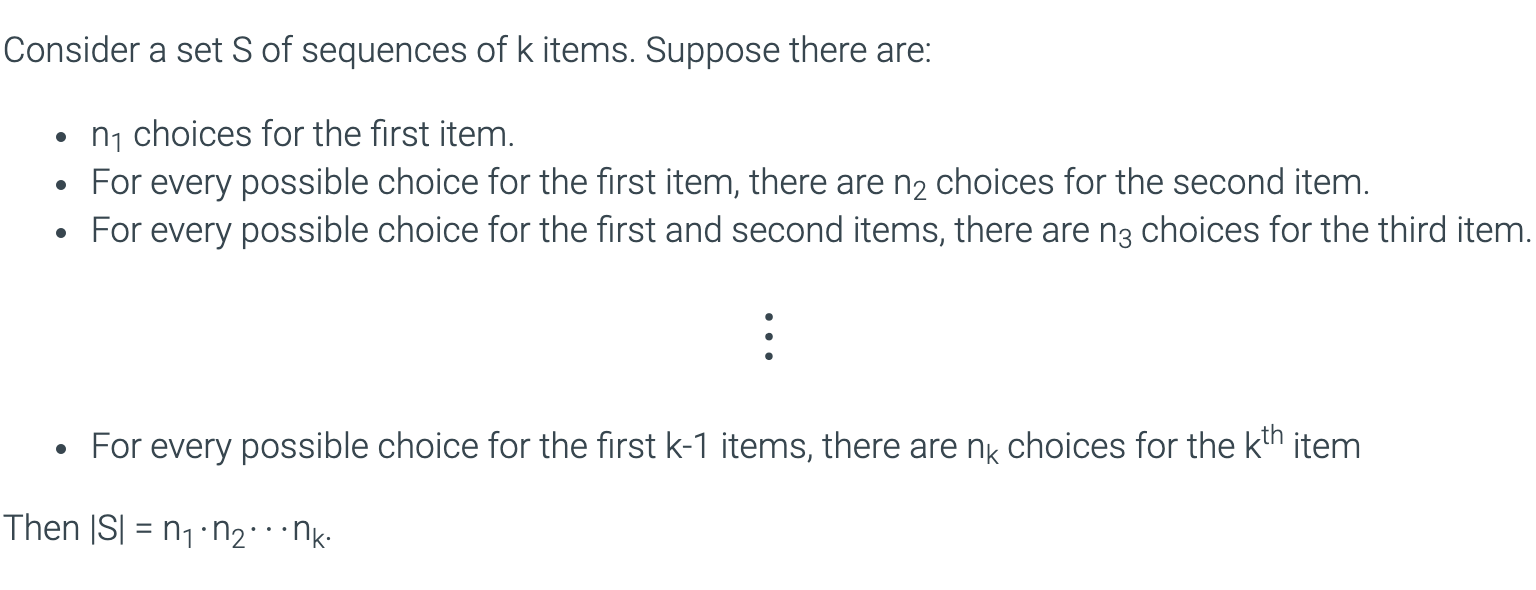
\includegraphics[scale=0.5]{general} 
  \end{itemize}
  \item \topic{Counting permutations}
  \begin{itemize}
    \item Each character in a password is either a digit [0 -\ 9] or lowercase letter [a-z]. How many valid passwords are there with the given restriction (s)?
    \item Length is 15. No character repeats.
    \item[] \boxed{nPr (36, 15)} 
    \item Length is 14. No character repeats. Starts with: t
    \item[] \boxed{nPr (35, 14)}
    \item Length is 17. No character repeats. Starts with: i0
    \item[] \boxed{nPr (34, 15)}
    \item Length is 15. No character repeats. Must contain: e
    \item[] \boxed{nPr (15, 1) * nPr (35, 14)}
    \item Length is 11. No character repeats. Must contain: i, 8, 3, 5
    \item[] 4 already chosen characters with 11 possible positions: nPr (11, 4)
    \item[] Then, permute 7 from 32 characters: nPr (32, 7)
    \item[] \boxed{nPr (11, 4) * nPr (32, 7)}
  \end{itemize}
  \item \topic{Counting subsets}
  \begin{itemize}
    \item A bit string contains 1's and 0's. How many different bit strings can be constructed given the restriction (s)?
    \item Length is 19.
    \item[] Each position has 2 possibilities: \(\boxed{2^{19}}\)
    \item Length is 17. Starts with: 111
    \item[] 17 -\ 3 positions remain, each with 2 possibilities: \(\boxed{2^{14}}\) 
    \item Length is 23. Has exactly five 0's.
    \item[] Choose five locations for 0's from 23 locations: \boxed{nCr (23, 5)} 
    \item Length is 22. Has exactly seven 0's. Starts with: 11
    \item[] First two locations already chosen.
    \item[] Choose seven locations for 0's from 20 locations: \boxed{nCr (20, 7)}  
    \item Length is 18. Has exactly six 1's in the first half. Has exactly two 1's in the second half.
    \item[] For first half, choose six 1's from 9: nCr (9, 6)
    \item[] For second half, choose two 1's from 9: nCr (9, 2)
    \item[] Then, combine: \boxed{nCr (9, 6) * nCr (9, 2)} 
  \end{itemize}
  \item \topic{Counting by complement}
  \begin{itemize}
    \item An auto dealer has 6 different cars and 5 different trucks. How many ways are there to select two vehicles?
    \item[] Choose 2 from 11 vehicles: \boxed{nCr (11, 2)} 
    \item A shop has 4 different shirts and 7 different jeans. How many ways are there to select 2 shirts?
    \item[] Choose 2 from 4 shirts: \boxed{nCr (4, 2)} 
    \item A shop has 6 different shirts and 8 different jeans. How many ways are there to select two items so that at least one jeans is chosen?
    \item[] First, choose 2 from all items: nCr (14, 2)
    \item[] Second, choose 2 from only shirts: nCr (6, 2)
    \item[] Finally, subtract only shirts from all item: \boxed{nCr (14, 2) -\ nCr (6, 2)}
    \item An auto dealer has 5 different cars and 7 different trucks. How many ways are there to select three vehicles so that at least one truck is chosen?
    \item[] First, choose 3 from all vehicles: nCr (12, 3)
    \item[] Second, choose 3 from only cars: nCr (5, 3) 
    \item[] Finally, subtract only cars from all vehicles: \boxed{nCr (12, 3) -\ nCr (5, 3)} 
  \end{itemize}
  \item \topic{Permutations with repetitions}
  \begin{itemize}
    \item A \textbf{permutation with repetition} is an ordering of a set of items in which some of the items may be identical to each other.
    \item[] 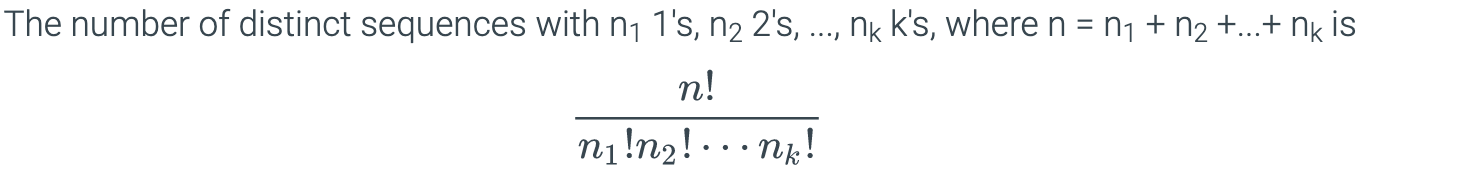
\includegraphics[scale=0.5]{perm} 
  \end{itemize}
  \item \topic{Counting multisets}
  \begin{itemize}
    \item A \textbf{multisets} is a collection that can have multiple instances of the same kind of item
  \end{itemize}
  \item \topic{Inclusion-exclusion principle}
  \begin{itemize}
    \item The principle of \textbf{inclusion-exclusion} is a technique for determining the cardinality of the union of sets that uses the cardinality of each individual set as well as the cardinality of their intersections.
    \item Given two sets: A and B. A has 8 elements. B has 5. How many elements are there in total?
    \item[] \(\vert A \vert \) = 8,  \(\vert B \vert \) = 5, \(\vert A \bigcap B \vert \) = 4
    \item[] \(\vert A \bigcup B \vert \) = \(\vert A \vert \) + \(\vert B \vert \)  \( - \vert A \bigcap B \vert \) = 8 + 5 -\ 4 = \boxed{\red{9}}
    \item Kate plays basketball 2 out of the 7 days of the week. How many possible schedules are there to play basketball on Wednesday or Tuesday or both.
    \item[] Define W to be the set of schedules in which Kate plays basketball on Wednesday.
    \item[] Define T to be the set of schedules in which Kate plays basketball on Tuesday.
    \item[] If Kate plays basketball on Wednesday, there are 6 remaining days from which to select the other day.
    \item[] If Kate plays basketball on Tuesday, there are 6 remaining days from which to select the other day.
    \item[] So \(\vert W \vert \) = \(\binom{6}{1}\) = 6 and \(\vert T \vert \) = \(\binom{6}{1}\) = 6
    \item[] There is only 1 way in which we select both: \(\vert W \bigcap T \vert \) =  \(\binom{5}{1}\) = 1 
    \item[] The number of schedules in which Kate plays basketball on Wednesday or Tuesday or both is:
    \item[] \(\vert W \bigcup T \vert \) = \(\vert W \vert \) + \(\vert T \vert \)  \( - \vert W  \bigcap T \vert \) = 6 + 6 -\ 1 = \boxed{\red{11}}
  \end{itemize}
\end{enumerate}


\clearpage
\begin{center}
  \large\textsc{\imp{Graphs}}
\end{center}
\begin{enumerate}
  \item \topic{Introduction to graphs} Directed graphs were introduced in the context of relations. Here we are concerned with \textbf{undirected graphs}. In an undirected graph, the edges are unordered pairs of vertices, which is useful for modeling relationships that are symmetric.
  A graph consists of a pair of sets (V, E), where V is a set of vertices and E is a set of edges. A graph is \textbf{finite} if the vertex set is finite. This material will only be concerned with finite graphs. A single element of V is called a \textbf{vertex} and is usually represented pictorially by a dot with a label. Each edge in E is a set of two vertices from V and is drawn as a line connecting the two vertices. In the graph below, the vertex set is V = \{a, b, c, d, e\}. The graph has six edges.
  \textbf{Parallel edges} are multiple edges between the same pair of vertices. Imagine a graph whose vertex set is a set of cities and whose edges are roads connecting pairs of cities. It is possible for there to be two different roads between the same two cities. In defining graphs with parallel edges, it would be important to have an additional label besides the two endpoints to specify an edge in order to distinguish between different parallel edges. A graph can also have a \textbf{self-loop} which is an edge between a vertex and itself. The graph below has two parallel edges between vertices a and b. There is also a self-loop at vertex c.
  \begin{itemize}
    \item[] 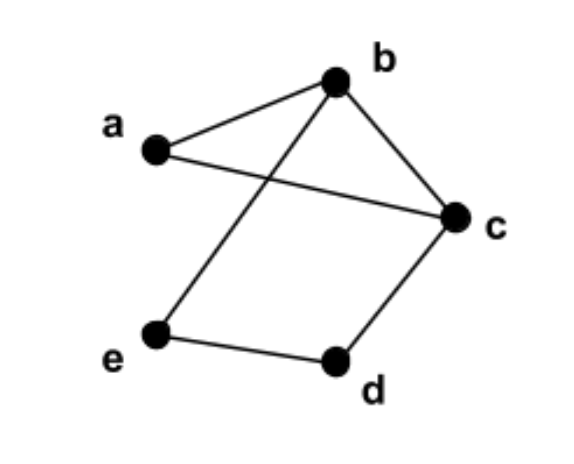
\includegraphics[scale=0.5]{graph}
    \item If there is an edge between two vertices, they are said to be \textbf{adjacent}. In the graph above, d and e are adjacent, but d and b are not adjacent.
    \item Vertices b and e are the \textbf{endpoints} of edge \{b, e\}. The edge \{b, e\} is \textbf{incident} to vertices b and e.
    \item A vertex c is a \textbf{neighbor} of vertex b if and only if \{b, c\} is an edge. In the graph above, the neighbors of b are the vertices a, c, and e.
    \item In a simple graph, the \textbf{degree} of a vertex is the number of neighbors it has. In the graph above, the degree of b is 3 and the degree of vertex a is 2. The degree of vertex b is denoted by deg (b).
    \item The \textbf{total degree} of a graph is the sum of the degrees of all of the vertices. The total degree of the graph above is 2 + 3 + 3 + 2 + 2 = 12.
    \item[] 
  \end{itemize}
  \item \topic{Graph representations}
  \begin{itemize}
    \item In the \textbf{adjacency list} representation of a graph, each vertex has a list of all its neighbors. Note that since the graph is undirected if vertex a is in b's list of neighbors, then b must also be in a's list of neighbors.
    \item The \textbf{matrix} representation for a graph with n vertices is an n by n matrix whose entries are all either 0 or 1, indicating whether or not each edge is present. If the matrix is labeled M, then \(M_{i,j} \) denotes the entry in row i and column j. For a matrix representation, the vertices of the graph are labeled with integers in the range from 1 to n. Entry \(M_{i,j=1} \) if and only if \{i, j\} is an edge in the graph. Since the graph is undirected, \(M_{i,j} \) = \(M_{j,i} \) because \{i, j\} and \{j, i\} refer to the same edge which is either present in the graph or not. Thus the matrix representation of an undirected graph is symmetric about the diagonal, meaning that it is a mirror image of itself along the diagonal extending from the upper left corner to the lower right corner.
  \end{itemize}
  \item \topic{Graph isomorphism}: Two graphs are said to be \textbf{isomorphic} if there is a correspondence between the vertex sets of each graph such that there is an edge between two vertices of one graph if and only if there is an edge between the corresponding vertices of the second graph. The graphs are not identical but the vertices can be relabeled so that they are identical.
  \begin{itemize}
    \item Let G = (V, E) and G' = (V',E').  G and G' are isomorphic if there is a bijection f: V → V' such that for every pair of vertices x, y \(\in \) V, \{x, y\} \(\in \) E if and only if \( \{f(x), f(y)\} \) \(\in \) E'. The function f is called an \textbf{isomorphism} from G to G'.
  \end{itemize}
  \item \topic{Walks, trails, circuits, paths, and cycles}:
  \begin{itemize}
    \item A \textbf{walk} from \(v_0 \) to \(v_l \) in an undirected graph G is a sequence of alternating vertices and edges that starts and ends with a vertex:\\ 
    \(\langle \blu{v_{0}},\red{\{v_{0},v_{1} \}}, \blu{v_{1}}, \red{\{v_{1}, v_{2} \}}, \blu{v_{1},\ldots,v_{l-1}}, \red{\{v_{l-1}, v_{l} \}}, \blu{v_{l}} \rangle \)
    \item The vertices just before and after each edge are the two endpoints of that edge.
    \item Since the edges in a walk are completely determined by the vertices, a walk can also be denoted by the sequence of vertices: \(\langle \blu{v_{0}, v_{1},\ldots, v_{l}} \rangle \)
    \item The sequence of vertices is a walk only if \( \{v_{i-1}, v_i\} \) \(\in \) E for each i = 1, 2,\(\ldots \),l. Two consecutive vertices \(\ldots \), \( v_{i-1}, v_i \), \(\ldots \) in a walk represent an occurrence of the edge \( \{v_{i-1}, v_i\} \) in the walk.
    \item The \textbf{length} of a walk is l, the number of edges in the walk.
    \item An \textbf{open walk} is a walk in which the first and last vertices are not the same. A \textbf{closed walk} is a walk in which the first and last vertices are the same.
    \item A \textbf{trail} is an open walk in which no edge occurs more than once.
    \item A \textbf{circuit} is a closed walk in which no edge occurs more than once.
    \item A \textbf{path} is a trail in which no vertex occurs more than once.
    \item A \textbf{cycle} is a circuit of length at least 1 in which no vertex occurs more than once, except the first and last vertices which are the same.
  \end{itemize}
  \item \topic{Graph connectivity}: In an undirected graph, if there is a path from vertex v to vertex w, then there is also a path from w to v. The two vertices, v and w, are said to be \textbf{connected}. A vertex is always considered to be connected to itself. If the graph represents a road or communication network, then it is very desirable for every pair of vertices to be connected. The property of being connected can be extended to sets of vertices and the entire graph:
  \begin{itemize}
    \item A set of vertices in a graph is said to be connected if every pair of vertices in the set is connected.
    \item A graph is said to be connected if every pair of vertices in the graph is connected, and is \textbf{disconnected} otherwise.
    \item A \textbf{connected component} is a maximal set of vertices that is connected. The word ``maximal'' means that if any vertex is added to a connected component, then the set of vertices will no longer be connected.
    \item A vertex that is not connected with any other vertex is called an \textbf{isolated vertex} and is therefore a connected component with only one vertex.
    \item An undirected graph G is \textbf{k-vertex-connected} if the graph contains at least k + 1 vertices and remains connected after any k -\ 1 vertices are removed from the graph. The \textbf{vertex connectivity} of a graph is the largest k such that the graph is k-vertex-connected. The vertex connectivity of a graph G is denoted \(k(G)\).
    \item An undirected graph G is \textbf{k-edge-connected} if it remains connected after any k -\ 1 edges are removed from the graph. The \textbf{edge connectivity} of a graph is the largest k such that the graph is k-edge-connected. The edge connectivity of a graph G is denoted \(\lambda (G)\).
  \end{itemize}
  \item \topic{Euler circuits and trails}
  \begin{itemize}
    \item An \textbf{Euler circuit} in an undirected graph is a circuit that contains every edge and every vertex. Note that a circuit, by definition, has no repeated edges, so an Euler circuit contains each edge exactly once.
    \item If an undirected graph G has an Euler circuit, then G is connected and every vertex in G has an even degree.
    \item If an undirected graph G is connected and every vertex in G has an even degree, then G has an Euler circuit.
    \item An undirected graph G has an Euler circuit if and only if G is connected and every vertex in G has even degree.
    \item An \textbf{Euler trail} is an open trail that includes each edge. Note that a trail, by definition, has no repeated edges, so an Euler trail contains each edge exactly once. In an open trail, the first and last vertices are not equal. As with Euler circuits, there is a simple set of conditions that characterize when an undirected graph has an Euler trail.
    \item An undirected graph G has an Euler trail if and only if G is connected and has exactly two vertices with odd degree.
  \end{itemize}
  \item \topic{Hamiltonian cycles and paths}
  \begin{itemize}
    \item A \textbf{Hamiltonian cycle} in an undirected graph is a cycle that includes every vertex in the graph. Note that a cycle, by definition, has no repeated vertices or edges, except for the vertex which is at the beginning and end of the cycle. Therefore, every vertex in the graph appears exactly once in a Hamiltonian cycle, except for the vertex which is at the beginning and end of the cycle.
    \item A \textbf{Hamiltonian path} in an undirected graph is a path that includes every vertex in the graph. Note that a path, by definition, has no repeated vertices or edges, so every vertex appears exactly once in a Hamiltonian path.
    \item[] 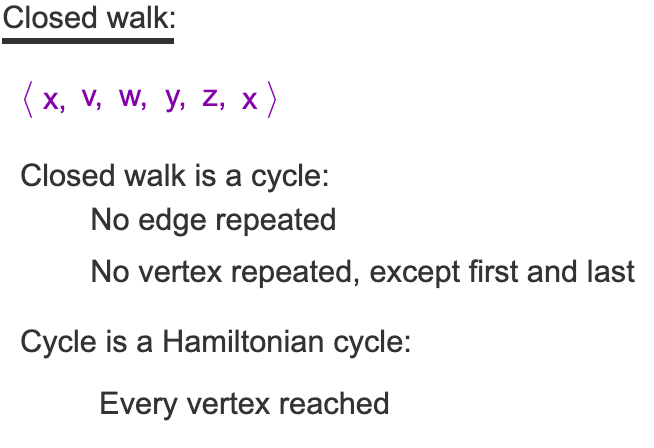
\includegraphics[scale=0.5]{closed1}
    \item[] 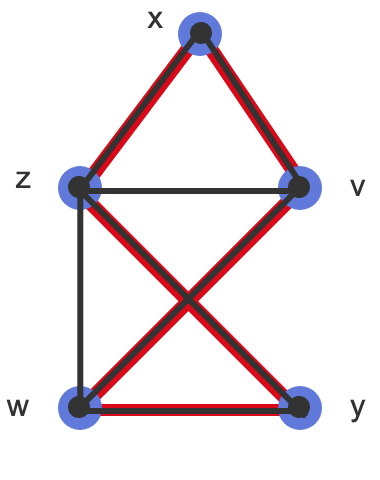
\includegraphics[scale=0.5]{closed}
    \item[] 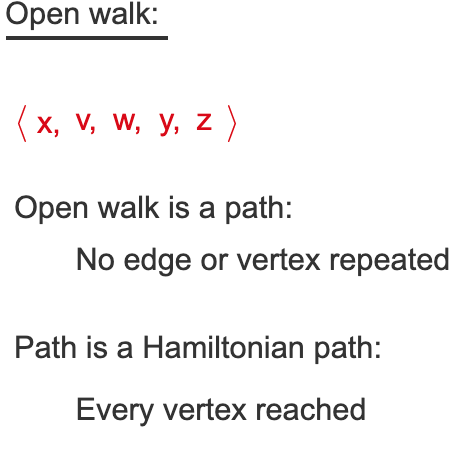
\includegraphics[scale=0.5]{open1} 
    \item[] 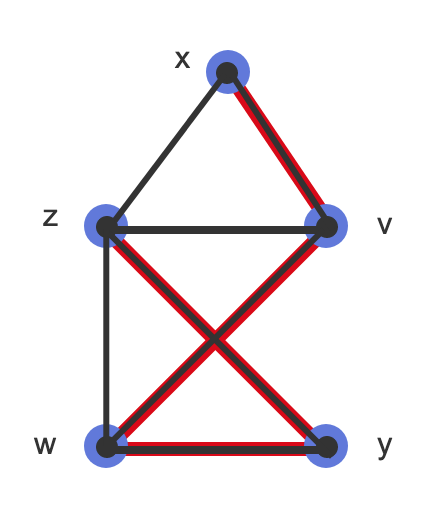
\includegraphics[scale=0.5]{open}    
  \end{itemize}
  \item \topic{Planar graphs}
  \begin{itemize}
    \item Graph G\\V = \{ a, b, c, d, e \} \\E = \{ \{ a, b \}, \{ b, c \}, \{ c, d \}, \{ d, a \}, \{ a, c \}, \{ b, d \}, \{ e, a \}, \{ e, b \} \}
    \item[] 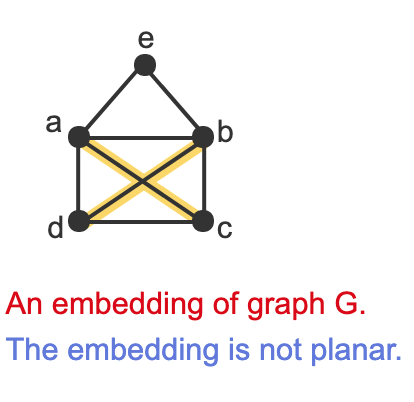
\includegraphics[scale=0.5]{planar1}
    \item[] 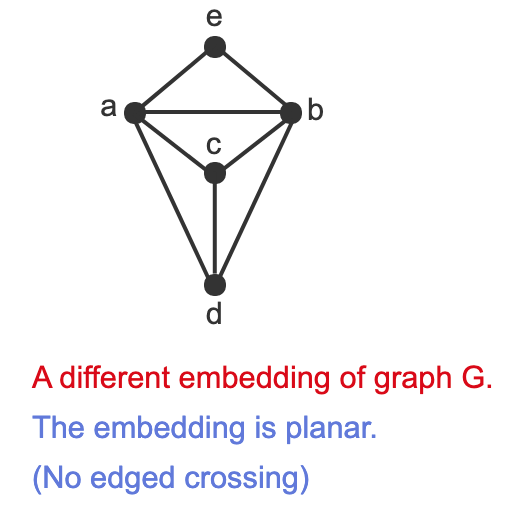
\includegraphics[scale=0.5]{planar2}
  \end{itemize}
  \item \topic{Graph coloring}
  \begin{itemize}
    \item Let G = (V, E) be an undirected graph and C a finite set of colors. A \textbf{valid coloring} of G is a function f: V → C such that for every edge \{x, y\} \(\in \) E, \(f(x) \neq f(y)\). If the size of the range of function f is k, then f is called a \textbf{k-coloring} of G.
    \item The \textbf{greedy coloring algorithm}:
    \item Number the set of possible colors. Assume that there is a very large supply of different colors, even though they might not all be used.
    \item Order the vertices in any arbitrary order.
    \item Consider each vertex v in order:
    \begin{itemize}
      \item Assign v a color that is different from the color of v's neighbors that have already been assigned a color. When selecting a color for v, use the lowest numbered color possible.
    \end{itemize}
  \end{itemize}
\end{enumerate}


\clearpage
\begin{center}
  \large\textsc{\imp{Trees}}
\end{center}
\begin{enumerate}
  \item \topic{Introduction to trees} -\ A \textbf{tree} is an undirected graph that is connected and has no cycles.
  The tree on the left is called a \textbf{free tree} because there is no particular organization of the vertices and edges. The tree on the right is called a \textbf{rooted tree}. The vertex at the top of the drawing is designated as the \textbf{root} of the tree. The remaining vertices are organized according to their distance from the root. The distance between two vertices in an undirected graph is the number of edges in the shortest path between the two vertices. The \textbf{level} of a vertex is its distance from the root. The \textbf{height} of a tree is the highest level of any vertex. The tree on the right has height 3.
  \item[] 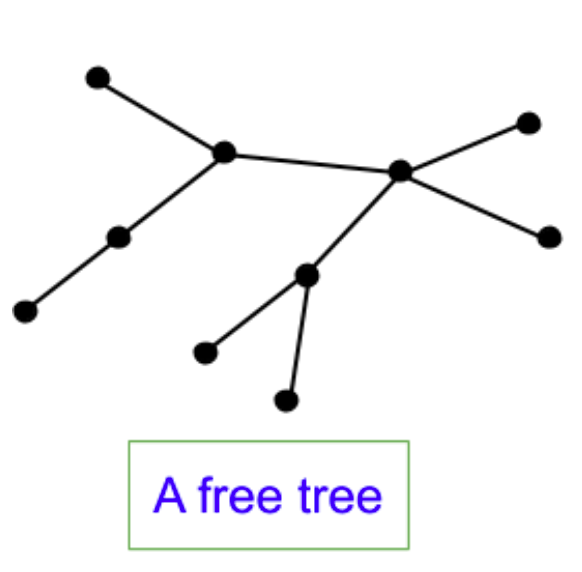
\includegraphics[scale=0.5]{freetree}
  \item[] 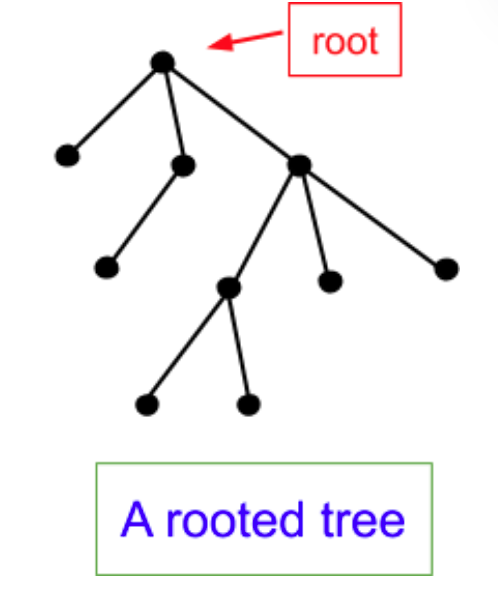
\includegraphics[scale=0.5]{rootedtree}
  \item[] 
  \item[] 
  \begin{itemize}
    \item[] 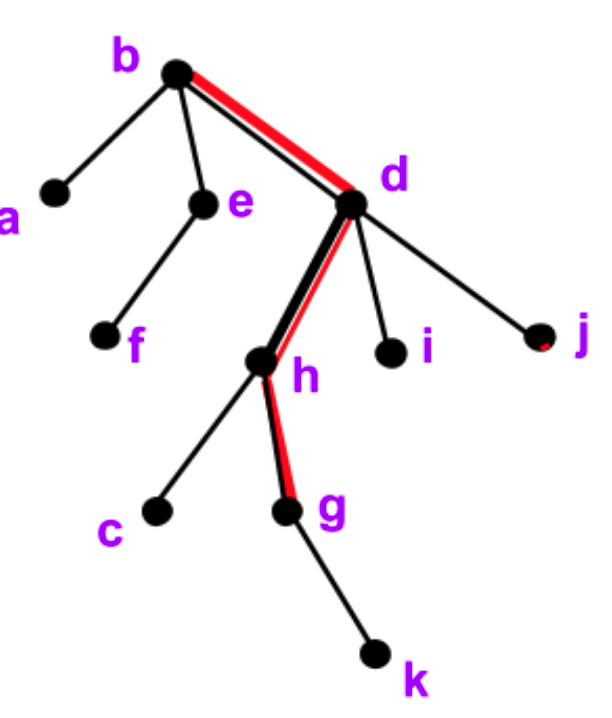
\includegraphics[scale=0.5]{tree}
    \item Every vertex in a rooted tree T has a unique \textbf{parent}, except for the root which does not have a parent. The parent of vertex v is the first vertex after v encountered along the path from v to the root. (Ex: The parent of vertex g is h.) 
    \item Every vertex along the path from v to the root (except for the vertex v itself) is an ancestor of vertex v. (Ex: The \textbf{ancestors} of vertex g are h, d, and b.)
    \item If v is the parent of vertex u, then u is a \textbf{child} of vertex v. (Ex: Vertices c and g are the children of vertex h.)
    \item If u is an ancestor of v, then v is a \textbf{descendant} of u. (Ex: The descendants of vertex h are c, g, and k.)
    \item A \textbf{leaf} is a vertex which has no children. (Ex: The leaves are a, f, c, k, i, and j.)
    \item Two vertices are \textbf{siblings} if they have the same parent. (Ex: Vertices h, i, and j are siblings because they have the same parent, which is vertex d.)
    \item A \textbf{subtree} rooted at vertex v is the tree consisting of v and all v's descendants. (Ex: The subtree rooted at h includes h, c, g, and k and the edges between them.)
  \end{itemize} 
  \item \topic{Properties of trees} -\ The definitions for parent and child vertices in rooted trees make use of the fact that every vertex has a unique path to the root. There is, in fact, a unique path between any pair of vertices in a tree. The theorem below applies to free trees as well as rooted trees.
  \textbf{Theorem}: There is a unique path between every pair of vertices in a tree.
  \begin{itemize}
    \item \textbf{Proof}. A tree is defined to be a connected graph with no cycles. Because every tree is connected, there is at least one path between every pair of vertices. It remains to establish that there is at most one path between every pair of vertices. The proof is by contrapositive. We assume that there is a pair of vertices u and v such that there are two distinct paths between u and v and then show that the graph must have a cycle (and therefore can not be a tree).
    \item[] 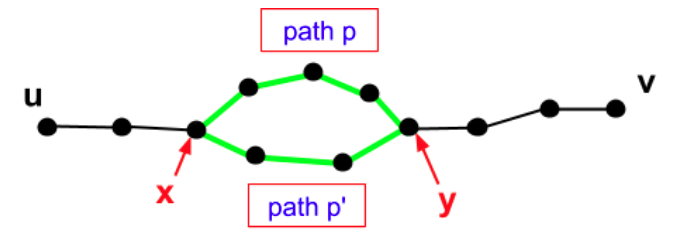
\includegraphics[scale=0.5]{t1}
    \item Let p and p' be the two distinct paths between u and v. Find the first place where the two paths differ. Let x be the vertex just before the point where the two paths diverge. Follow path p until it hits a vertex y that is also contained in p'. (Both paths end up at v, so there has to be a point where the two paths come together). The portion of the path p between x and y and the portion of the path p' between x and y form a cycle. 
    \item[]
    \item The term leaf is defined in rooted trees as a vertex with no children. A leaf has a natural definition in free trees as well. A leaf of a free tree is a vertex of degree 1. There is one technicality: if a free tree has only one vertex, then that vertex is a leaf. A vertex is an internal vertex if the vertex has degree at least two. The following theorem gives a lower bound on the number of leaves in a free tree:
    \item[] \textbf{Theorem}: Any free tree with at least two vertices has at least two leaves.
    \item \textbf{Proof}. Find the longest path p in the tree. Let u and v be the first and last vertices in the path. Suppose u is not a degree 1 vertex. (The same argument will hold for v). Then there is an edge e that is incident to u and not part of the path p.
    \item[] 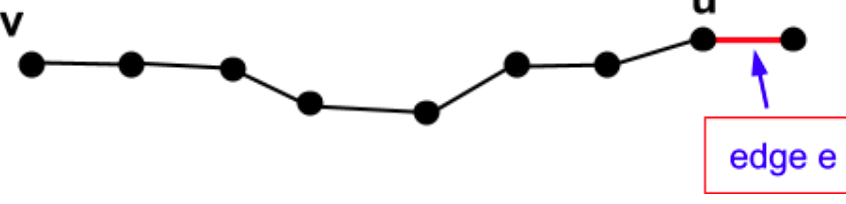
\includegraphics[scale=0.5]{t2}
    \item If the other endpoint of e, that is not vertex u, is part of the path p, then the graph has a cycle and is not a tree. The path p can be extended by adding e along with the other endpoint of e. The fact that the path p can be extended contradicts the assumption that p was the longest path in the tree.
    \item \textbf{Theorem}: Let T be a tree with n vertices and m edges, then m = n -\ 1
    \item \textbf{Proof}. The proof is by induction on the number of vertices. The base case is where n = 1. If T has one vertex, then it is has no edges. Then m = 0 = n -\ 1.
    \item For the inductive step, assume the theorem holds for trees with n -\ 1 vertices and prove that it holds for trees with n vertices. Consider an arbitrary tree T with n vertices. Since n \(\leq \) 2, by the previous theorem, the tree has at least two leaves. Let v be one of the leaves. Remove v from T along with the edge e incident to v. The resulting graph (call it T') is also a tree and has n-1 vertices.
    \item[] 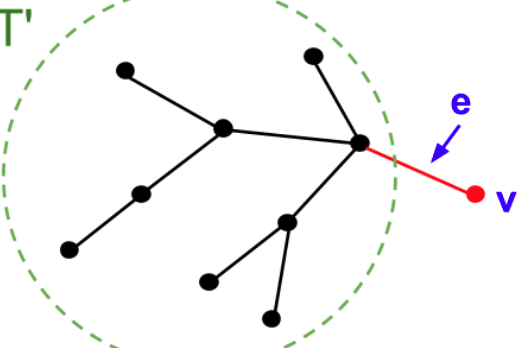
\includegraphics[scale=0.5]{t3}
    \item By the induction hypothesis, The number of edges in T' is (n -\ 1) -\ 1 = n -\ 2. T has exactly one more edge than T', because only edge e was removed from T to get T'. Therefore the number of edges in T is n -\ 2 + 1 = n -\ 1 
  \end{itemize}
  \item \topic{Tree traversals}
  \begin{itemize}
    \item Pseudocode for pre-order traversal.
    \item[] 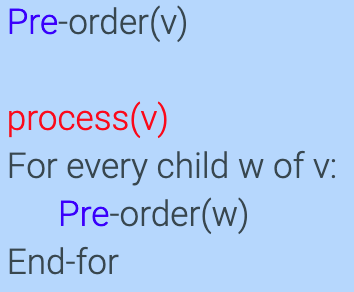
\includegraphics[scale=0.5]{pre}
    \item[] 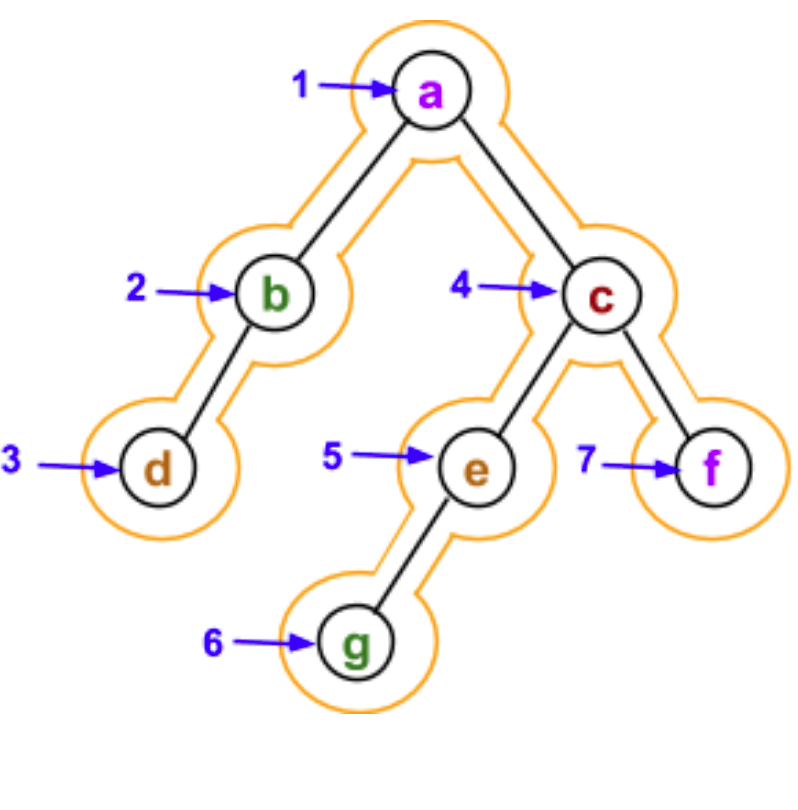
\includegraphics[scale=0.5]{pre1} 
    \item[] 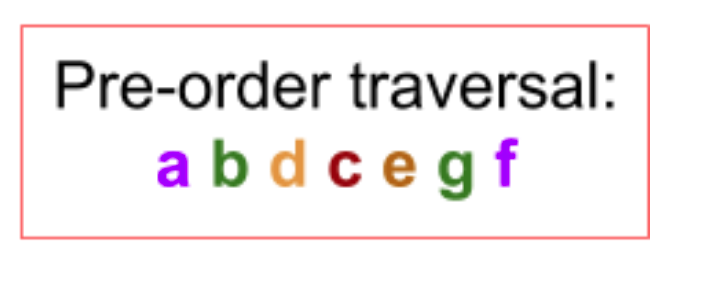
\includegraphics[scale=0.5]{pre2} 
    \item Pseudocode for post-order traversal.
    \item[] 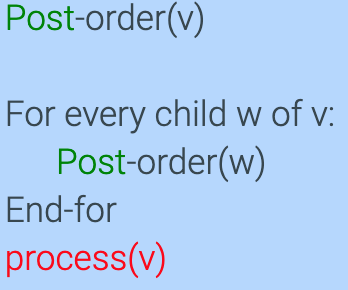
\includegraphics[scale=0.5]{post}
    \item[] 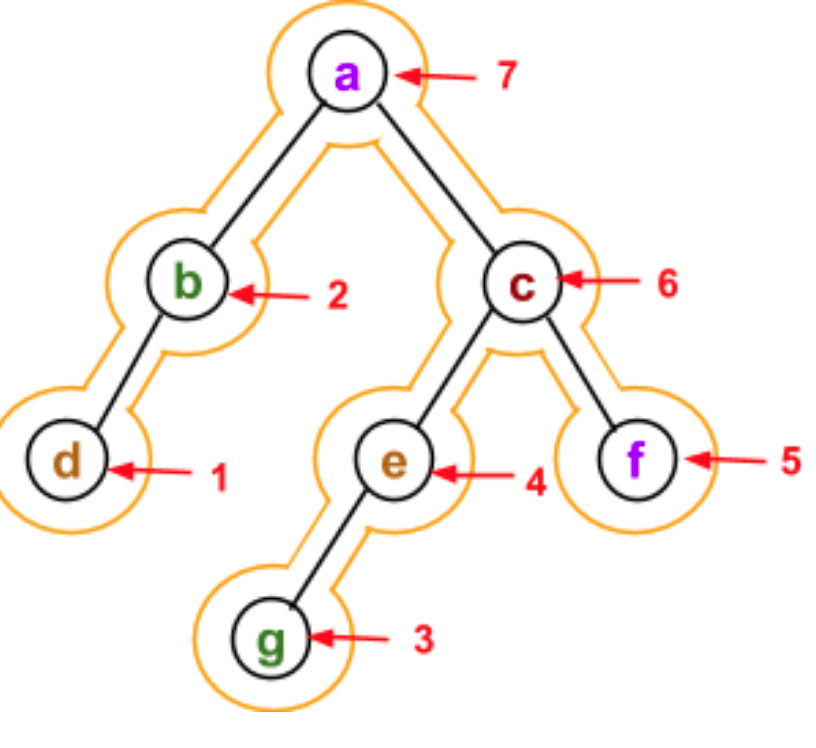
\includegraphics[scale=0.5]{post1}
    \item[] 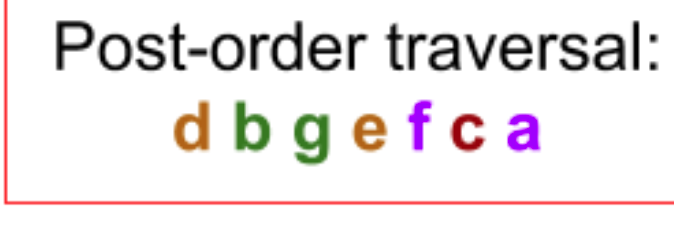
\includegraphics[scale=0.5]{post2} 
  \end{itemize}
  \item \topic{Spanning trees and graph traversals}
  \begin{itemize}
    \item A spanning tree of a connected graph G is a subgraph of G which contains all the vertices in G and is a tree.
    \item \textbf{Depth-First Search}
    \item[] 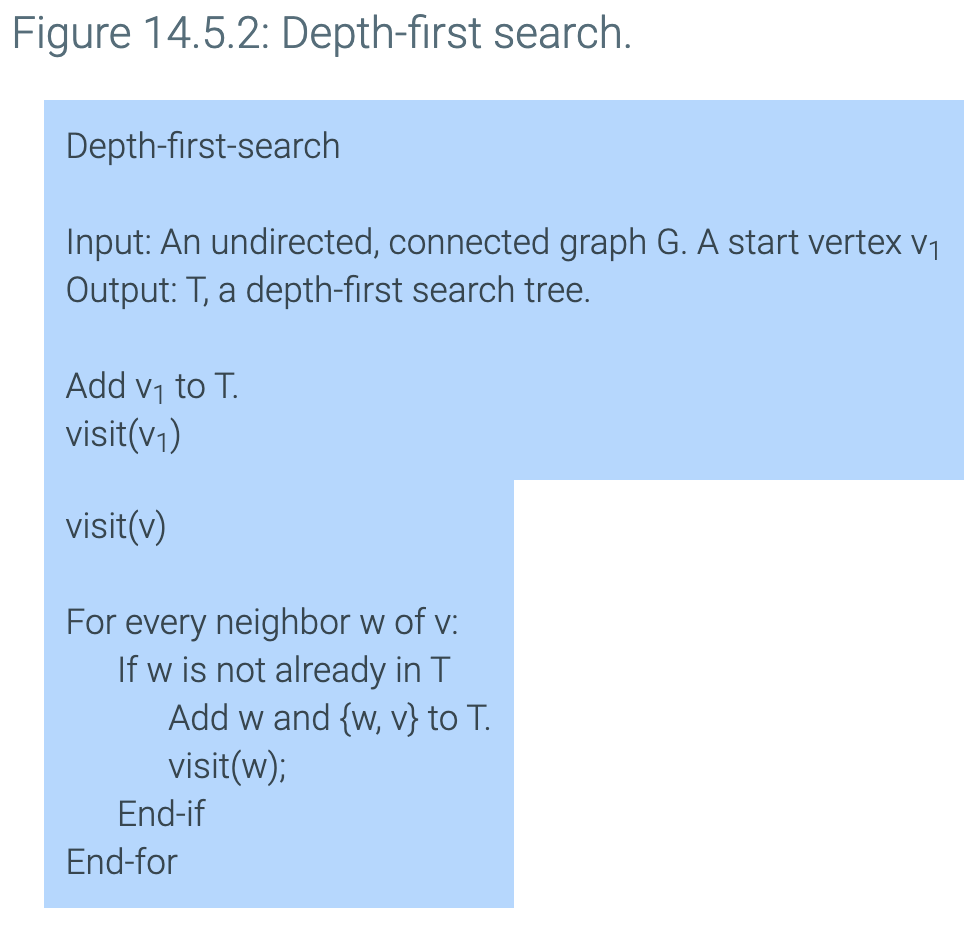
\includegraphics[scale=0.5]{dfs}
     \item \textbf{Breadth-first-search}
    \item[] 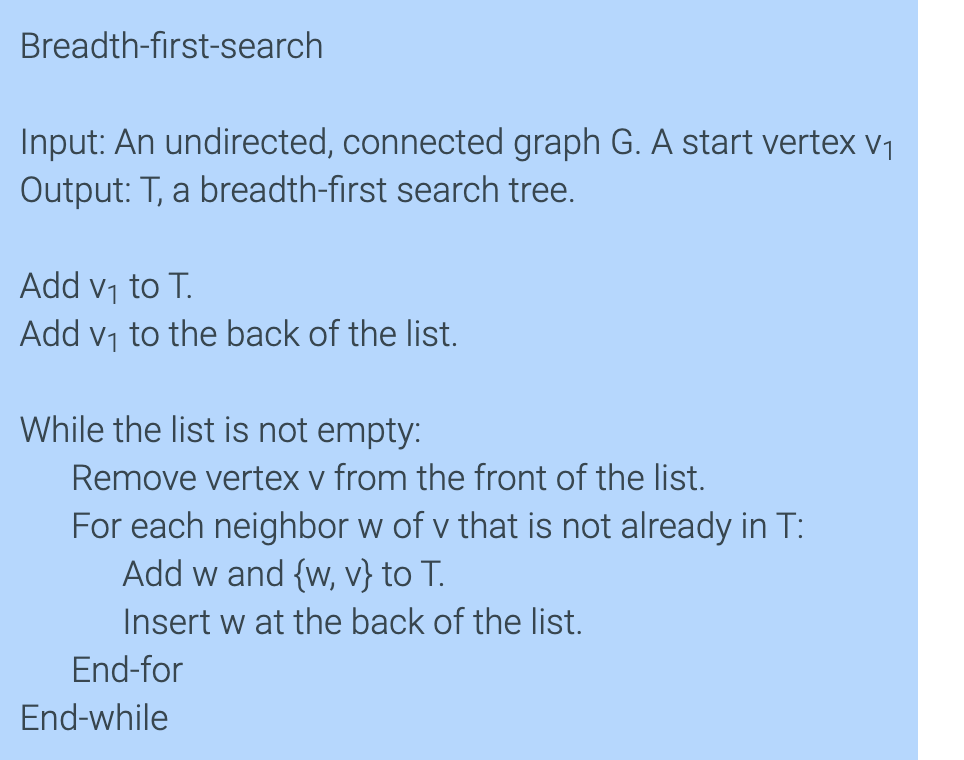
\includegraphics[scale=0.5]{bfs}
  \end{itemize}
  \item \topic{Minimum spanning trees}: A spanning tree of a graph specifies a subset of the edges that provides connectivity between every pair of vertices while minimizing the number of edges included. Every spanning tree of a graph with n nodes has n-1 edges, so there is no reason to prefer one spanning tree over another if the only goal is to include as few edges as possible.
  \begin{itemize}
    \item A \textbf{weighted graph} is a graph G = (V, E), along with a function w: E → R. The function w assigns a real number to every edge.
    \item A \textbf{minimum spanning tree (MST)} of a weighted graph, is a spanning tree T of G whose weight is no larger than any other spanning tree of G.
    \item A graph can have more than one minimum spanning tree because there can be more than one spanning tree with the same weight. In the extreme case, if the weight of every edge is 1, then every spanning tree has weight n -\ 1 and every spanning tree is also a minimum spanning tree.
    \item \textbf{Prim's algorithm} finds a minimum spanning tree
  \end{itemize}
\end{enumerate}
\end{document}